% !TEX root = ../CategoricalCoDesign.tex
\section{Monotonicity is a fact of life}
\subsection{Monotone maps}
\AC{Add some motivation from design. E.g. generalization of "non-decreasing" and "non-increasing" from real numbers to partial orders}
\begin{definition}[Monotone map]
A monotone map between two posets
$\tup{A, \leq_A}$ and $\tup{B, \leq_B}$ is a map that preserves the ordering, in the sense that 
\begin{equation}
 a \leq_A b \quad \Imp \quad f(a) \leq_B f(b).
\end{equation}

A monotone map is an \emph{isomorphism} if the other direction
of the implication holds as well:
\begin{equation}
 a \leq_A b \quad \Leftrightarrow \quad f(a) \leq_B f(b).
\end{equation}
\end{definition}

\begin{remark}
Given a preorder $A$, $\id_A$ is monotone, since for $a_1,a_2\in A$, one has:
\begin{equation}
a_1\leq_A a_2 \Imp a_1=a_1\then \id_A \leq_A a_2\then \id_A = a_2.
\end{equation}
\end{remark}



\begin{example}
In \cref{ex:hasseinclusion} we presented the poset arising from the power set of a set $A=\{a,b,c\}$ and ordered via subset inclusion. The map $\vert \cdot \vert \colon \powerset(A)\to \mathbb{N}$ (cardinality), is a monotone map:
\begin{center}
\includesag{40_dpcatfig_exmonotone}
\end{center}
\end{example}
Note that monotonicity is a compositional property.

\begin{lemma}Given three posets $A, B, C$ and two monotone maps $f\colon A
\to B$ and  $g\colon B \to C$, the composite map $f\then g\colon  A \to C$ is
monotone as well.
\end{lemma}
\begin{proof}
Consider $a_1,a_2 \in A$, $b_1,b_2\in B$. We have 
\begin{equation}
\begin{aligned}
        a_1\leq_A a_2 &\Imp f(a_1)\leq_Q f(a_2)\\ 
        b_1\leq_B b_2 &\Imp g(b_1)\leq_C g(b_2).
\end{aligned}
\end{equation}
By substituting the above, one has
\begin{equation}
    a_1\leq_A a_2 \Imp (f\then g)(a_1) \leq_C (f\then g)(a_2),
\end{equation}
which is the monotonicity condition for $(f\then g)$.
\end{proof}

\begin{lemma}
Consider a discrete poset $A$ and a poset $B$. Any map $f\colon A\to B$ is monotone.
\end{lemma}
\begin{proof}
Since $A$ is a discrete poset, one has
\begin{equation}
    a_1\leq_A a_2 \iff a_1=a_2.
\end{equation}
Therefore, one has
\begin{equation}
    a_1\leq_A a_2 \Imp a_1=a_2 \Imp f(a_1)=f(a_2) \Imp f(a_1)\leq_B f(a_2).
\end{equation}
\end{proof}
Unless indicated otherwise, in this paper all maps between two posets
are assumed to be monotone or will turn out to be monotone.

\subsection{A poset as a category}

A single poset $\tup{P, \leq}$ can be described as a category, in which
each point $p\in P$ is an object, and there is a morphism between
$p$ and $q$ if and only if $p \leq q$. This is a ``thin'' category, which means that there is at most one morphism
between two objects: For any $p,q\in P$, there exist only one relation $p\leq q$ in $P$. The identity morphism is given by the reflexivity of posets, i.e. for any $p\in P$, $p\leq p$. Furthermore, composition is given by transitivity of posets, i.e. for $p,q,r \in P$, $p\leq q$ and $q\leq r$ implies $p\leq r$.

\begin{example}
Let's revisit \cref{ex:hasseinclusion}, in which we had a poset $\powerset{\{a,b,c\}}$ with order given by the inclusion:
\begin{center}
\begin{tikzcd}
& \{a,b,c\} & \\
\{a,b\}\arrow{ru} & \{a,c\}\arrow{u} & \{b,c\}\arrow{lu}\\
\{a\} \arrow{u}\arrow{ru}& \{b \}\arrow{lu}\arrow{ru} & \{c \}\arrow{u}\arrow{lu} \\
&\varnothing \arrow{lu}\arrow{ru} \arrow{u}&
\end{tikzcd}
\end{center}
This is a category $\CatC$, with $\ObC=\powerset{\{a,b,c\}}$ and morphisms given by the inclusion. Note that we omit to draw self-arrows for the identity morphisms. Composition is given by the transitivity of the poset. Note, for instance, that since $\{a\}\subset \{a,b\}$ and $\{a,b\} \subset \{a,b,c\}$, we can say $\{a\}\subset \{a,b,c\}$.
\end{example}




\subsection{The category $\Pos$ of posets and monotone maps}
In the previous section, we described a poset as a category, where the objects are elements of the poset and the morphisms are given by the poset order. In this section, we want to lift this concept and describe a category in which the objects are posets themselves, and the morphisms are monotone functions between them. This category is called $\Pos$.

\begin{definition}[Category $\Pos$]
    The category $\Pos$ is defined by:
    \begin{compactenum}
    \item \emph{Objects}: The objects of this category are all posets.
    \item \emph{Morphisms}: The morphisms between any pair of posets $X, Y$
    are the monotone maps from $X$ to $Y$.
    \item \emph{Identity morphism}:  The identity morphism for the poset $X$
    is the identity function $\text{Id}_X$.
    \item \emph{Composition operation}: The composition operation is function
    composition.
    \end{compactenum}
\end{definition}

Occasionally we will write $f \colon A \to_{\Pos} B$ to emphasize that a monotone map between posets is a morphism in the category of posets, called~$\Pos$. Note that morphisms in $\Pos$ are morphisms between posets, which we previously defined as categories. The notion of ``morphisms between categories'' is formally described through functors.

\begin{shaded}
\begin{definition}[Functor]
\label{def:functor}
Given the categories $\CatC$ and $\CatD$, to specify a \emph{functor} $F\colon \CatC\to \CatD$ from $\CatC$ to $\CatD$,
\begin{compactenum}
    \item for every object $c\in \ObC,$ one specifies and object $F(c)\in \ObD$;
    \item for every morphism $f\colon c_1\to c_2$ in $\CatC$, one specifies a morphism $F(f)\colon F(c_1)\to F(c_2)$ in $\CatD$.
\end{compactenum}
The above constituents must satisfy the following two properties:
\begin{compactenum}[(a)]
    \item For every object $c\in \ObC$, one has $F(\id_c)=\id_{F(c)}$.
    \item For every three objects $c_1,c_2,c_3 \in \ObC$ and two morphisms $f\in \CatC(c_1,c_2)$, $g\in \CatC(c_2,c_3)$, the equation $F(f\then g)=F(f)\then F(g)$ holds in $\CatD$.
\end{compactenum}
\end{definition}

\begin{definition}[Full and faithful functors]
\label{def:functorfullfaith}
A functor $F\colon \CatC \to \CatD$ is \emph{full} (resp.\ \emph{faithful} if for each pair of objects $x,y\in \CatC$, the function
\begin{equation}
    F\colon \CatC(x,y)\to \CatD(F(x),F(y))
\end{equation}
is surjective (resp.\ injective).
\end{definition}
\end{shaded}

\begin{lemma}
A monotone function $F$ between posets $P,Q \in \Pos$ is a functor between the categories $P$ and $Q$.
\end{lemma}
\begin{proof}
We start by specifying the functor $F$ by specifying its action on objects (elements of a poset) and on morphisms (order relation). A monotone function maps each element of a poset $p\in P$ to $F(p) \in Q$, and, given two posets $P$ and $Q$, it guarantees that for $p_1,p_2\in P$, $F(p_1),F(p_2)\in Q$,  $p_1\leq p_2$ implies $f(p_1)\leq f(p_2)$. We now need to check the two functor properties. First, consider the identity morphism for $p\in P$, namely $p\leq p$. The application of the functor results in the condition $f(p)\leq F(p)$, which is the identity morphism on $Q$. Finally, given three elements $p_1,p_2,p_3\in P$ and two morphisms $p_1\leq p_2$ and $p_2\leq p_3$, by applying the functor to the morphism composition $p_1\leq p_3$ one obtains $F(p_1)\leq F(p_3)$, which is the same as $F(p_1)\leq F(p_2)$ and $F(p_2)\leq F(p_3)$.
\end{proof}



\subsection{Composing posets}

\AC{ At this point you can re-do the constructions}
\subsubsection{Product of posets}

\begin{definition}[Product of posets]
Given two posets $\tup{A, \leq_A}$
and  $\tup{B, \leq_B}$, the product poset is $\tup{A \times B, \leq_{A\times B}}$, where $A \times B$ is the Cartesian product of two sets (\cref{def:cartesian-product}) and the order $\leq_{A\times B}$ is given by
\begin{equation}
        \langle a_1, b_1 \rangle
        \leq_{A\times B}
        \langle a_2, b_2 \rangle
        \quad
        \Leftrightarrow
        \quad
        ( a_1 \leq_A a_2) \wedge
        (b_1 \leq_B b_2).
    \end{equation}
\end{definition}

\begin{example}
Consider now the two posets
\begin{center}
\includesag{40_exposet_1}
\end{center}
Their product is depicted as
\begin{center}
\includesag{40_exposet_2}
\end{center}
\end{example}

\subsubsection{Disjoint union of posets}

\todo{intro}

\begin{definition}[Disjoint union of posets]
Given two posets $\tup{A, \leq_A} $ and $\tup{B, \leq_B} $,
we can define their disjoint union $\tup{ A + B, \leq_{A + B}}$, where $A + B$
is the disjoint union of two sets (\cref{def:disjoint-union}), and the
order $\leq_{A + B}$ is given by:
\begin{equation}
    x \leq_{A + B} y \quad\equiv\quad
    \begin{cases}
        x \leq_A y, & \text{if } x,y \in A, \\
        x \leq_B y, & \text{if } x,y \in B, \\
        \false,  & \text{otherwise}.
    \end{cases}
\end{equation}
\end{definition}


\begin{figure}[h!]
    \centering
    \includesag{40_disjoint_union}
    %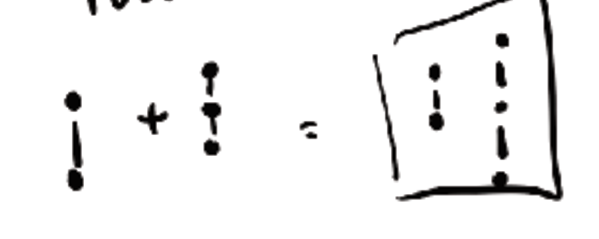
\includegraphics[scale=0.33]{dpcatfig_poset_disjoint_union}
    \caption{\label{fig:poset-coproduct}}
\end{figure}


\AC{Add example here.}


\paragraph{A note on pre-orders}

    The theory of design problems can be easily generalized to preorders, i.e. posets without the antisymmetry property; this means that there could be two elements $a$ and $b$ such that $a\leq b$ and $a \geq b$ but $a \neq b$.

    \begin{equation}
    \includesag{80_preorder}
    \end{equation}

    This is actually common in practice. For example, if the order relation comes from human judgement, such as customer preference, all bets are off regarding the consistency of the relation. We will only refer to posets for two reasons:
    \begin{compactenum}
        \item The exposition is smoother;
        \item Given a preorder, computation will always involve passing to the poset representation.
    \end{compactenum}
    This means that, given a preorder, we can consider the poset of its equivalence classes, by means of the following equivalence relation:
    \begin{equation}
        a \simeq b \quad \equiv \quad (a \leq b) \wedge (b \leq a).
    \end{equation}%
    
